% ============================================================
%  IoT Project Report Template
%  Compile with: pdflatex (run twice so the contents/lists update)
%  LOGO: put your college logo in the same folder as this file
%        and name it  college_logo.png  (or change \logofile below).
%        If the file is missing, a labelled empty box is shown instead.
% ============================================================
\documentclass[12pt,a4paper]{report}

\usepackage[a4paper,left=1.5in,right=1in,top=1in,bottom=1in]{geometry}
\usepackage{graphicx}
\usepackage{booktabs}
\usepackage{longtable}
\usepackage{tabularx}
\usepackage{array}
\usepackage{setspace}
\usepackage{fancyhdr}
\usepackage{listings}
\usepackage{xcolor}
\usepackage{caption}
\usepackage[hidelinks]{hyperref}
\usepackage{float}
\usepackage{tikz}
\usetikzlibrary{positioning,arrows.meta,shapes.geometric,calc}

\onehalfspacing

% ---------- FILL THESE IN ----------
\newcommand{\projecttitle}{AERIS: Aviation Experimental Recording and
Instrumentation System}
\newcommand{\studentnames}{Ashwin Kumar (1262242905)\\Anvi Singh Parihar (1262242193)}
\newcommand{\guidename}{Mrs.\ Sujata Jagadale}
\newcommand{\hodname}{Dr.\ B. M. Patil}
\newcommand{\department}{Department of Computer Engineering}
\newcommand{\collegename}{School of Computer Engineering and Technology}
\newcommand{\universityname}{MITWPU}
\newcommand{\degreename}{Bachelor of Technology}
\newcommand{\academicyear}{2026--2027}
\newcommand{\logofile}{logo.png}
\newcommand{\rupee}{Rs.}  % currency label used in the BOM
% -----------------------------------

% Logo: shows the image if present, otherwise an empty box
\newcommand{\collegelogo}[1]{%
  \IfFileExists{\logofile}%
    {\includegraphics[height=#1]{\logofile}}%
    {\fbox{\parbox[c][#1][c]{#1}{\centering\small Place college\\logo here}}}%
}

% Code listing style
\lstset{basicstyle=\ttfamily\footnotesize,breaklines=true,frame=single,
        numbers=left,numberstyle=\tiny,backgroundcolor=\color{gray!8}}

% Diagram styles
\tikzset{
  blk/.style={draw,rounded corners=2pt,align=center,font=\footnotesize,minimum height=0.9cm,inner sep=3pt,fill=gray!8},
  hw/.style={blk,fill=blue!8},
  sw/.style={blk,fill=green!8},
  net/.style={blk,fill=orange!10},
  arr/.style={-{Stealth[length=2mm]},thick},
  lbl/.style={font=\scriptsize,align=center},
  dec/.style={diamond,draw,aspect=2.2,align=center,font=\footnotesize,inner sep=1pt,fill=yellow!10},
  term/.style={blk,rounded corners=8pt,fill=gray!20},
  pin/.style={font=\scriptsize}
}

% Header/footer
\pagestyle{fancy}
\fancyhf{}
\fancyhead[L]{\small AERIS}
\fancyhead[R]{\small\department}
\fancyfoot[C]{\thepage}
\renewcommand{\headrulewidth}{0.4pt}

% Make chapter pages keep the footer page number
\fancypagestyle{plain}{\fancyhf{}\fancyfoot[C]{\thepage}\renewcommand{\headrulewidth}{0pt}}

\begin{document}

% ============================================================
%  FRONT MATTER
% ============================================================
\pagenumbering{roman}

% ---------------- TITLE PAGE ----------------
\begin{titlepage}
\thispagestyle{empty}
\centering
{\Large\bfseries \universityname\par}
\vspace{0.4cm}
{\Large\bfseries \collegename\par}
\vspace{0.3cm}
{\large \department\par}
\vspace{0.8cm}

\collegelogo{3.2cm}\par
\vspace{1cm}

{\large A Project Report on\par}
\vspace{0.4cm}
{\LARGE\bfseries \projecttitle\par}
\vspace{0.8cm}

{\large Submitted in partial fulfilment of the requirements for the degree of\par}
{\large\bfseries \degreename\par}
\vspace{0.8cm}

{\large Submitted by\par}
\vspace{0.3cm}
{\large\bfseries \studentnames\par}
\vspace{0.8cm}

{\large Under the guidance of\par}
{\large\bfseries \guidename\par}
\vfill
{\large Academic Year \academicyear\par}
\end{titlepage}

% ---------------- CERTIFICATE ----------------
\newpage
\thispagestyle{empty}
\begin{center}
\collegelogo{2.4cm}\par\vspace{0.4cm}
{\Large\bfseries \collegename\par}
{\large \department\par}
\vspace{1cm}
{\Large\bfseries CERTIFICATE\par}
\end{center}
\vspace{0.8cm}

\noindent This is to certify that the project report entitled
\textbf{``\projecttitle''} is a bonafide work carried out by

\begin{center}
\textbf{\studentnames}
\end{center}

\noindent in partial fulfilment of the requirements for the award of the degree of
\textbf{\degreename} in \textbf{\department} of \textbf{\universityname}
during the academic year \textbf{\academicyear}, under my supervision and guidance.

\vspace{2.2cm}
\noindent
\begin{tabularx}{\textwidth}{XXX}
\rule{4cm}{0.4pt} & \\
\textbf{\guidename}\\
Project Guide & \\
\end{tabularx}

\vspace{1.5cm}
\noindent Date: \hrulefill \\[0.3cm]
Place: \hrulefill

% ---------------- DECLARATION ----------------
\chapter*{Declaration}
\addcontentsline{toc}{chapter}{Declaration}
We declare that the project report entitled \textbf{``\projecttitle''}
is our own work. We did this work under the guidance of \guidename. We did not
submit this work for a different degree or diploma. We identify all sources of
information in the report.

\vspace{2cm}
\begin{flushright}
\studentnames
\end{flushright}

% ---------------- ACKNOWLEDGEMENT ----------------
\chapter*{Acknowledgement}
\addcontentsline{toc}{chapter}{Acknowledgement}
We thank our project guide, \guidename, for her guidance and support during this project.

We thank \hodname, Head of the \department, and the faculty members of the
department for the facilities and support that we used in this work.
We thank \collegename\ for the opportunity to do this project.

We also thank our families and friends for their support.

\vspace{1.5cm}
\begin{flushright}
\studentnames
\end{flushright}

% ---------------- ABSTRACT ----------------
\chapter*{Abstract}
\addcontentsline{toc}{chapter}{Abstract}
\emph{Flight-test data acquisition systems are expensive, and their designs are not open. Thus, students cannot examine the full data path from a sensor to a ground station. AERIS (Aviation Experimental Recording and Instrumentation System) is a low-cost IoT unit that shows this data path. An STM32F446RE microcontroller reads an MPU-6500 inertial measurement unit at 100 Hz and a BMP280 barometer at 10 Hz through I\textsuperscript{2}C. The STM32 calculates a pressure altitude and sends 20 telemetry packets per second to an ESP8266 through UART. Each packet is a JSON line with a sequence number, a timestamp and an XOR checksum. The ESP8266 publishes the packets to a Mosquitto MQTT broker through Wi-Fi. A Python Dash dashboard shows live plots and diagnostics and records the data to CSV files. The two microcontrollers have separate tasks, so network failures do not stop sampling. The firmware recovers from sensor and bus faults without a reset, and it sends invalid values as null. In a hardware test, the system sent 575 packets at 20.0 Hz with no packet loss. All 33 automatic tests pass. AERIS is a teaching and laboratory unit, not a certified aircraft instrument.}

\vspace{0.5cm}
\noindent\textbf{Keywords:} IoT, Flight Instrumentation, STM32, ESP8266, MQTT, Telemetry

% ---------------- INDEX / LISTS ----------------
\tableofcontents
\clearpage
\listoffigures
\addcontentsline{toc}{chapter}{List of Figures}
\clearpage
\listoftables
\addcontentsline{toc}{chapter}{List of Tables}

\chapter*{List of Abbreviations}
\addcontentsline{toc}{chapter}{List of Abbreviations}
\begin{tabular}{@{}ll@{}}
BOM   & Bill of Materials\\
CSV   & Comma-Separated Values\\
FTI   & Flight Test Instrumentation\\
GPIO  & General Purpose Input/Output\\
HAL   & Hardware Abstraction Layer\\
I\textsuperscript{2}C & Inter-Integrated Circuit\\
IMU   & Inertial Measurement Unit\\
IoT   & Internet of Things\\
JSON  & JavaScript Object Notation\\
LED   & Light-Emitting Diode\\
MCU   & Microcontroller Unit\\
MQTT  & Message Queuing Telemetry Transport\\
QNH   & Sea-level reference pressure for altitude\\
RTOS  & Real-Time Operating System\\
UART  & Universal Asynchronous Receiver-Transmitter\\
\end{tabular}

% ============================================================
%  MAIN MATTER
% ============================================================
\clearpage
\pagenumbering{arabic}

% ---------------- CHAPTER 1 ----------------
\chapter{Introduction}
\section{Background}
A flight-test instrumentation system reads sensors on an aircraft, adds a timestamp to each sample and sends the data to a ground station. AERIS is a small IoT model of this system for teaching and laboratory use. It is not a certified aircraft instrument.

\section{Problem Statement}
Commercial flight-test systems are expensive, and their designs are not open. Thus, students cannot examine how such a system collects, sends and shows sensor data. A low-cost, open unit is necessary to show the full data path and to record the data for analysis.

\section{Objectives}
\begin{itemize}
\item Read the IMU and barometer at fixed rates, and calculate a pressure altitude.
\item Send numbered, timestamped packets through Wi-Fi to a dashboard that shows, records and monitors the data.
\end{itemize}

\section{Scope and Limitations}
The scope is the full path from the sensor drivers to the dashboard. AERIS does not include aircraft integration, certification, roll and pitch calculation or storage on the device.

% ---------------- CHAPTER 2 ----------------
\chapter{Literature Survey}
\section{Existing Systems and Related Work}
\begin{itemize}
\item \textbf{Commercial FTI systems:} Companies such as Curtiss-Wright and Safran supply flight-test systems for commercial and military aircraft. These systems are reliable and have high sample rates. They are expensive, and their designs are not open.
\item \textbf{Open-source autopilots:} Pixhawk boards with ArduPilot or PX4 firmware record IMU and barometer data \cite{ardupilot}. The data path is part of a complex flight-control system. Thus, it is difficult to use as a simple teaching example.
\item \textbf{Generic IoT sensor nodes:} One ESP8266 or ESP32 reads the sensors and also runs Wi-Fi. A Wi-Fi reconnection or a TCP delay stops the sensor reads, so the sample timing is not regular. Most of these nodes do not check frames and do not recover from sensor faults.
\end{itemize}

\section{Comparison with Existing Systems}
\begin{table}[H]
\centering
\caption{Comparison of existing solutions}
\label{tab:comparison}
\small
\begin{tabularx}{\textwidth}{|>{\hsize=0.9\hsize}X |>{\hsize=1.0\hsize}X |>{\hsize=1.1\hsize}X |>{\hsize=1.0\hsize}X|}
\toprule
\textbf{System / Paper} & \textbf{Technology} & \textbf{Advantages} & \textbf{Limitations}\\
\midrule
Commercial FTI systems & Special hardware, PCM and Ethernet buses & Certified, reliable, high sample rates & High cost, closed design\\
\midrule
Pixhawk with ArduPilot \cite{ardupilot} & STM32F4/F7, NuttX RTOS, IMU and barometer & Open source, good flight logs & Data path is part of flight control, difficult to study\\
\midrule
Generic IoT nodes & ESP8266 or ESP32, Arduino & Very low cost, fast to build & Wi-Fi delays sampling, no frame checks, no fault recovery\\
\midrule
AERIS (this project) & STM32F446RE, ESP8266, MQTT, Python dashboard & Two MCUs, fixed 100 Hz sampling, checked frames, open design & Not certified, for teaching only\\
\bottomrule
\end{tabularx}
\end{table}

\section{Gaps Addressed by This Project}
\begin{itemize}
\item \textbf{Separate measurement and networking:} The STM32 samples the sensors. The ESP8266 does only the networking. A network failure does not change the sample timing.
\item \textbf{Open design:} All code is available. A student can follow each sample from the sensor register to the CSV file.
\item \textbf{Visible faults:} The system counts each fault, lost packet and checksum error. It sends invalid data as \texttt{null}, not as zero.
\item \textbf{Low cost:} The hardware costs approximately \rupee~3000.
\end{itemize}

% ---------------- CHAPTER 3 ----------------
\chapter{System Analysis and Requirements}
\section{Functional and Non-Functional Requirements}
\subsection{Functional Requirements}
Requirements R1 to R5 in Table~\ref{tab:requirements} are functional: acquisition, processing, telemetry, display and logging, and commands.

\subsection{Non-Functional Requirements}
Requirements R6 to R9 are non-functional: isolation of sampling from the network, automatic recovery, reliability and data integrity.

\section{Requirements Specification Table}
\begin{table}[H]
\centering
\caption{Requirements specification}
\label{tab:requirements}
\small
\begin{tabularx}{\textwidth}{|p{1.0cm}|X|l|l|X|}
\toprule
\textbf{Req ID} & \textbf{Description} & \textbf{Type} & \textbf{Priority} & \textbf{Verification}\\
\midrule
\textbf{R1} & IMU at 100 Hz, barometer at 10 Hz & Functional & High & Status message counters \\ \hline
\textbf{R2} & Pressure altitude from a set QNH & Functional & Medium & Manual calculation \\ \hline
\textbf{R3} & 20 Hz packets with timestamp, sequence number and checksum & Functional & High & Recorded CSV data \\ \hline
\textbf{R4} & Live dashboard and CSV recording & Functional & High & Tests and inspection \\ \hline
\textbf{R5} & QNH command to the STM32 & Functional & Medium & \texttt{command\_ack} event \\ \hline
\textbf{R6} & Sampling continues during network failure & Non-functional & High & Stop the broker \\ \hline
\textbf{R7} & Sensor recovery in 1 s without reset & Non-functional & High & Disconnect a sensor \\ \hline
\textbf{R8} & Packet loss below 1\% & Non-functional & High & Sequence gaps \\ \hline
\textbf{R9} & Invalid values as \texttt{null} & Non-functional & High & Unit tests \\
\bottomrule
\end{tabularx}
\end{table}

\section{Hardware Requirements}
\begin{itemize}
\item STM32 Nucleo-F446RE board and ESP8266 NodeMCU (or Wemos D1 mini) board.
\item MPU-6500 and BMP280 breakouts for 3.3 V, wires and two USB cables.
\item A computer on the same Wi-Fi network as the ESP8266.
\end{itemize}

\section{Software Requirements}
\label{sec:sw}
\begin{itemize}
\item STM32CubeIDE with the STM32 HAL (no RTOS).
\item Arduino IDE with the ESP8266 core 3.1.2 and PubSubClient 2.8.
\item Mosquitto, and Python 3 with Dash 4.4, Plotly 7.1, paho-mqtt 2 and pytest.
\end{itemize}

% ---------------- CHAPTER 4 ----------------
\chapter{System Design}
\section{Block Diagram}
\begin{figure}[H]
\centering
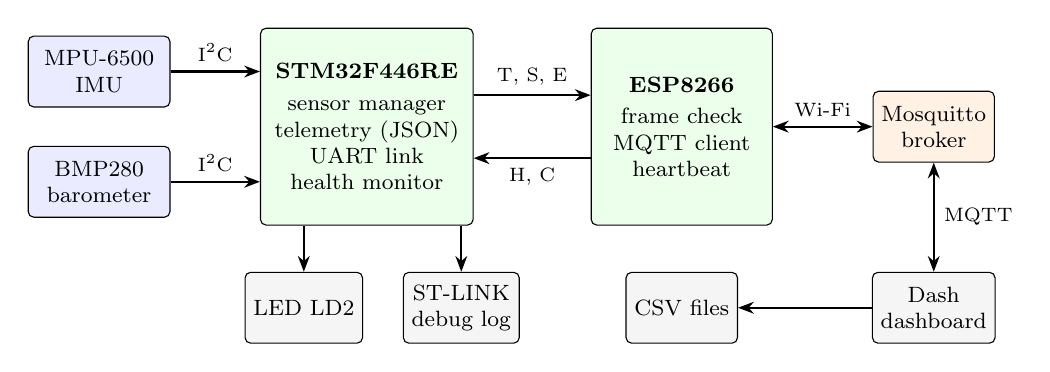
\begin{tikzpicture}
\node[hw,minimum width=1.8cm] (mpu) at (0,0) {MPU-6500\\IMU};
\node[hw,minimum width=1.8cm] (bmp) at (0,-1.4) {BMP280\\barometer};
\node[sw,minimum width=2.7cm,minimum height=2.5cm] (stm) at (3.4,-0.7) {\textbf{STM32F446RE}\\[2pt]sensor manager\\telemetry (JSON)\\UART link\\health monitor};
\node[sw,minimum width=2.3cm,minimum height=2.5cm] (esp) at (7.4,-0.7) {\textbf{ESP8266}\\[2pt]frame check\\MQTT client\\heartbeat};
\node[net] (brk) at (10.6,-0.7) {Mosquitto\\broker};
\node[blk] (dash) at (10.6,-3.0) {Dash\\dashboard};
\node[blk] (csv) at (7.4,-3.0) {CSV files};
\node[blk] (led) at (2.6,-3.0) {LED LD2};
\node[blk] (dbg) at (4.6,-3.0) {ST-LINK\\debug log};
\draw[arr] (mpu.east) -- node[lbl,above]{I\textsuperscript{2}C} (mpu.east -| stm.west);
\draw[arr] (bmp.east) -- node[lbl,above]{I\textsuperscript{2}C} (bmp.east -| stm.west);
\draw[arr] ([yshift=0.4cm]stm.east) -- node[lbl,above]{T, S, E} ([yshift=0.4cm]esp.west);
\draw[arr] ([yshift=-0.4cm]esp.west) -- node[lbl,below]{H, C} ([yshift=-0.4cm]stm.east);
\draw[arr,{Stealth[length=2mm]}-{Stealth[length=2mm]}] (esp) -- node[lbl,above]{Wi-Fi} (brk);
\draw[arr,{Stealth[length=2mm]}-{Stealth[length=2mm]}] (brk) -- node[lbl,right]{MQTT} (dash);
\draw[arr] (dash) -- (csv);
\draw[arr] (stm.south -| led) -- (led);
\draw[arr] (stm.south -| dbg) -- (dbg);
\end{tikzpicture}
\caption{System block diagram}
\label{fig:block_diagram}
\end{figure}

\section{IoT Architecture Layers}
\begin{enumerate}
\item \textbf{Perception:} MPU-6500 and BMP280 on one I\textsuperscript{2}C bus at 400 kHz.
\item \textbf{Edge:} The STM32 samples, checks and averages the data, and makes JSON packets.
\item \textbf{Network:} UART to the ESP8266, then MQTT through Wi-Fi to the broker.
\item \textbf{Application:} The Python dashboard shows, records and sends commands.
\end{enumerate}

\section{Circuit Diagram}
\begin{figure}[H]
\centering
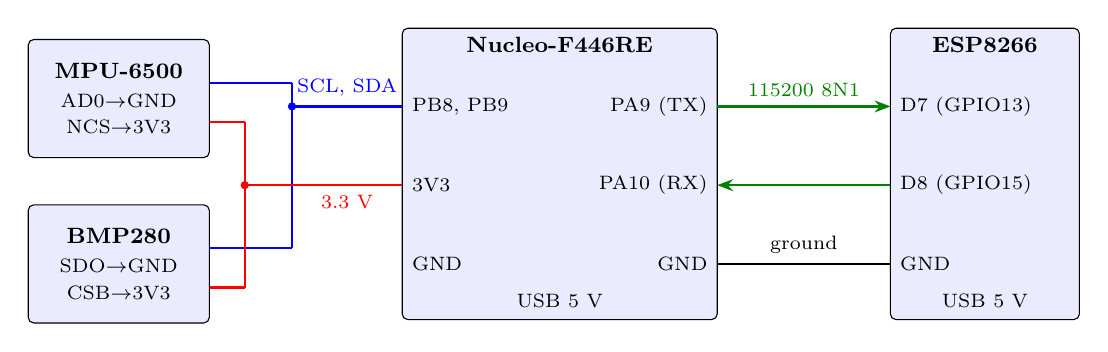
\begin{tikzpicture}
% Nucleo
\node[hw,minimum width=4.0cm,minimum height=3.7cm,anchor=north] (nuc) at (0,0) {};
\node[font=\footnotesize\bfseries,anchor=north] at (nuc.north) {Nucleo-F446RE};
\node[pin,anchor=west] at (-2.0,-1.0) {PB8, PB9};
\node[pin,anchor=west] at (-2.0,-2.0) {3V3};
\node[pin,anchor=west] at (-2.0,-3.0) {GND};
\node[pin,anchor=east] at (2.0,-1.0) {PA9 (TX)};
\node[pin,anchor=east] at (2.0,-2.0) {PA10 (RX)};
\node[pin,anchor=east] at (2.0,-3.0) {GND};
\node[pin,anchor=south] at ([yshift=1pt]nuc.south) {USB 5 V};
% Sensors
\node[hw,minimum width=2.3cm,minimum height=1.5cm] (mpu) at (-5.6,-0.9) {\textbf{MPU-6500}\\[1pt]\scriptsize AD0$\to$GND\\\scriptsize NCS$\to$3V3};
\node[hw,minimum width=2.3cm,minimum height=1.5cm] (bmp) at (-5.6,-3.0) {\textbf{BMP280}\\[1pt]\scriptsize SDO$\to$GND\\\scriptsize CSB$\to$3V3};
% ESP8266
\node[hw,minimum width=2.4cm,minimum height=3.7cm,anchor=north] (esp) at (5.4,0) {};
\node[font=\footnotesize\bfseries,anchor=north] at (esp.north) {ESP8266};
\node[pin,anchor=west] at (4.2,-1.0) {D7 (GPIO13)};
\node[pin,anchor=west] at (4.2,-2.0) {D8 (GPIO15)};
\node[pin,anchor=west] at (4.2,-3.0) {GND};
\node[pin,anchor=south] at ([yshift=1pt]esp.south) {USB 5 V};
% I2C bus
\draw[thick,blue] (-2.0,-1.0) -- (-3.4,-1.0);
\draw[thick,blue] (-3.4,-0.7) -- (-3.4,-2.8);
\draw[thick,blue] (-3.4,-0.7) -- (mpu.east |- 0,-0.7);
\draw[thick,blue] (-3.4,-2.8) -- (bmp.east |- 0,-2.8);
\fill[blue] (-3.4,-1.0) circle (1.5pt);
\node[pin,blue,above] at (-2.7,-1.0) {SCL, SDA};
% 3.3 V
\draw[thick,red] (-2.0,-2.0) -- (-4.0,-2.0);
\draw[thick,red] (-4.0,-1.2) -- (-4.0,-3.3);
\draw[thick,red] (-4.0,-1.2) -- (mpu.east |- 0,-1.2);
\draw[thick,red] (-4.0,-3.3) -- (bmp.east |- 0,-3.3);
\fill[red] (-4.0,-2.0) circle (1.5pt);
\node[pin,red,below] at (-2.7,-2.0) {3.3 V};
% UART and ground
\draw[thick,green!50!black,-{Stealth[length=2mm]}] (2.0,-1.0) -- node[pin,above]{115200 8N1} (4.2,-1.0);
\draw[thick,green!50!black,{Stealth[length=2mm]}-] (2.0,-2.0) -- (4.2,-2.0);
\draw[thick] (2.0,-3.0) -- node[pin,above]{ground} (4.2,-3.0);
\end{tikzpicture}
\caption{Circuit diagram (blue: I\textsuperscript{2}C, red: 3.3 V, green: UART)}
\label{fig:circuit_diagram}
\end{figure}

\section{Flowchart and Data Flow Diagram}
\begin{figure}[H]
\centering
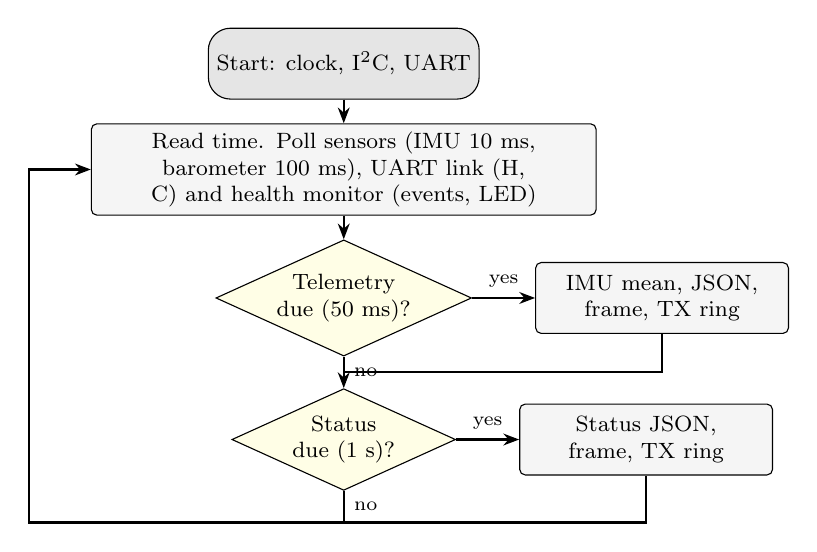
\begin{tikzpicture}[node distance=0.35cm]
\node[term] (s) {Start: clock, I\textsuperscript{2}C, UART};
\node[blk,below=0.3cm of s,text width=6.2cm] (p) {Read time. Poll sensors (IMU 10 ms, barometer 100 ms), UART link (H, C) and health monitor (events, LED)};
\node[dec,below=0.3cm of p] (d1) {Telemetry\\due (50 ms)?};
\node[blk,right=0.8cm of d1,text width=3.0cm] (b) {IMU mean, JSON, frame, TX ring};
\node[dec,below=0.4cm of d1] (d2) {Status\\due (1 s)?};
\node[blk,right=0.8cm of d2,text width=3.0cm] (st) {Status JSON, frame, TX ring};
\coordinate (m) at ($(d1.south)!0.5!(d2.north)$);
\coordinate (e) at ($(d2.south)+(0,-0.4)$);
\draw[arr] (s) -- (p);
\draw[arr] (p) -- (d1);
\draw[arr] (d1) -- node[lbl,above]{yes} (b);
\draw[arr] (d1) -- node[lbl,right]{no} (d2);
\draw[thick] (b) |- (m);
\draw[arr] (d2) -- node[lbl,above]{yes} (st);
\draw[thick] (st) |- (e);
\draw[thick] (d2.south) -- node[lbl,right]{no} (e);
\draw[arr] (e) -- ++(-4.0,0) |- (p.west);
\end{tikzpicture}
\caption{STM32 main loop flowchart}
\label{fig:system_flowchart}
\end{figure}

\begin{figure}[H]
\centering
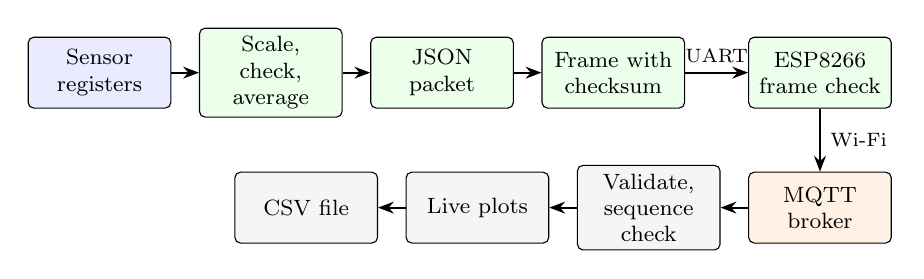
\begin{tikzpicture}[node distance=0.35cm]
\node[hw,text width=1.6cm] (a) {Sensor registers};
\node[sw,right=of a,text width=1.6cm] (b) {Scale, check, average};
\node[sw,right=of b,text width=1.6cm] (c) {JSON packet};
\node[sw,right=of c,text width=1.6cm] (d) {Frame with checksum};
\node[sw,right=0.8cm of d,text width=1.6cm] (e) {ESP8266 frame check};
\node[net,below=0.8cm of e,text width=1.6cm] (f) {MQTT broker};
\node[blk,left=of f,text width=1.6cm] (g) {Validate, sequence check};
\node[blk,left=of g,text width=1.6cm] (h) {Live plots};
\node[blk,left=of h,text width=1.6cm] (i) {CSV file};
\draw[arr] (a)--(b); \draw[arr] (b)--(c); \draw[arr] (c)--(d); \draw[arr] (d)--node[lbl,above]{UART}(e);
\draw[arr] (e)--node[lbl,right]{Wi-Fi}(f); \draw[arr] (f)--(g); \draw[arr] (g)--(h); \draw[arr] (h)--(i);
\end{tikzpicture}
\caption{Data flow of one telemetry sample}
\label{fig:data_flow_diagram}
\end{figure}

\section{Communication Protocol Selection}
\begin{itemize}
\item \textbf{I\textsuperscript{2}C:} Two wires for both sensors. Each transfer has a 5 ms timeout. Nine clock pulses and a STOP condition release a locked bus.
\item \textbf{UART:} 115200 baud, 8N1. Each frame is one ASCII line, \texttt{\$K:<json>*HH}, where \texttt{HH} is an XOR checksum (Table~\ref{tab:frames}). The \texttt{\$} lets the receiver find the next frame after an error.
\item \textbf{MQTT \cite{mqtt}:} A light publish-subscribe protocol on TCP. A retained last-will message tells the dashboard when the bridge is offline.
\end{itemize}

\begin{table}[H]
\centering
\caption{UART frame kinds and MQTT topics}
\label{tab:frames}
\small
\begin{tabularx}{\textwidth}{l l l X}
\toprule
\textbf{Kind} & \textbf{Direction} & \textbf{MQTT topic} & \textbf{Content}\\
\midrule
\texttt{T} & STM32 $\rightarrow$ ESP & \texttt{aeris/telemetry} & Sensor data, 20 Hz\\
\texttt{S} & STM32 $\rightarrow$ ESP & \texttt{aeris/status} & States and counters, 1 Hz\\
\texttt{E} & STM32 $\rightarrow$ ESP & \texttt{aeris/event} & State changes\\
\texttt{H} & ESP $\rightarrow$ STM32 & -- & Wi-Fi and MQTT state, 1 Hz\\
\texttt{C} & ESP $\rightarrow$ STM32 & \texttt{aeris/command} & Command from the dashboard\\
-- & ESP $\rightarrow$ broker & \texttt{aeris/status/esp} & Bridge diagnostics, 5 s, retained\\
\bottomrule
\end{tabularx}
\end{table}

\section{Component Selection Rationale}
\begin{table}[H]
\centering
\caption{Component selection comparison}
\label{tab:component_selection}
\small
\begin{tabularx}{\textwidth}{l X X}
\toprule
\textbf{Component Category} & \textbf{Candidates Evaluated} & \textbf{Selection Rationale \& Decision} \\
\midrule
\textbf{Microcontroller} & \textbf{Option A:} STM32F446RE (Selected)\newline \textbf{Option B:} Arduino Uno &
Cortex-M4 with a floating-point unit and 128 KB SRAM. The Uno has only 2 KB SRAM. \\
\addlinespace
\textbf{Sensor} & \textbf{Option A:} MPU-6500 (Selected)\newline \textbf{Option B:} MPU-9250 &
Has the six axes that the project needs. The MPU-9250 adds a magnetometer that is not used. \\
\addlinespace
\textbf{Comm. Module} & \textbf{Option A:} ESP8266 (Selected)\newline \textbf{Option B:} ESP32 &
Lower cost. The bridge does not process data, so the ESP32 performance is not necessary. \\
\bottomrule
\end{tabularx}
\end{table}

% ---------------- CHAPTER 5 ----------------
\chapter{Hardware Description}
\section{Microcontroller}
The STM32F446RE \cite{stm32} has a Cortex-M4 core with a floating-point unit, 512 KB flash and 128 KB SRAM. AERIS runs it at 84 MHz. USART2 sends the debug log to the ST-LINK USB port.

\section{Sensors and Actuators}
\begin{itemize}
\item \textbf{MPU-6500 \cite{mpu6500}:} Accelerometer and gyroscope. Settings: $\pm4$ g, $\pm500$ deg/s, 41 Hz low-pass filter, 100 Hz.
\item \textbf{BMP280 \cite{bmp280}:} Pressure and chip temperature. Settings: $\times16$ oversampling, IIR filter 16.
\item \textbf{Actuator:} LED LD2 shows the system state (Chapter~\ref{ch:manual}).
\end{itemize}

\section{Power Supply and Connectivity Modules}
Each board has its own USB supply, because the ESP8266 \cite{esp8266} has 300 mA peaks. All logic is 3.3 V. A transmit-only software UART on ESP8266 GPIO1 sends its debug log to USB.

\section{Pin Configuration}
\begin{table}[H]
\centering
\caption{Pin mapping}
\label{tab:pins}
\small
\begin{tabularx}{\textwidth}{lXll}
\toprule
\textbf{MCU Pin} & \textbf{Connected To} & \textbf{Protocol} & \textbf{Voltage}\\
\midrule
PB8, PB9 & Sensor SCL, SDA & I\textsuperscript{2}C1 & 3.3 V\\
PA9, PA10 & ESP8266 D7, D8 (GPIO13, 15) & USART1 TX, RX & 3.3 V\\
PA5 & LED LD2 & GPIO & 3.3 V\\
3V3, GND & Sensor power, NCS, CSB; AD0, SDO, common ground & Power & 3.3 V\\
\bottomrule
\end{tabularx}
\end{table}

\section{Bill of Materials (BOM)}
\begin{table}[H]
\centering
\caption{Bill of Materials}
\label{tab:bom}
\small
\begin{tabularx}{\textwidth}{llXlrrl}
\toprule
\textbf{S.No} & \textbf{Ref.} & \textbf{Description / Part No.} & \textbf{Qty} & \textbf{Unit (\rupee)} & \textbf{Total (\rupee)} & \textbf{Supplier}\\
\midrule
1 & U1 & STM32 Nucleo-F446RE & 1 & 2000 & 2000 & Online\\
2 & U2 & ESP8266 NodeMCU 1.0 & 1 & 300 & 300 & Online\\
3 & S1 & MPU-6500 breakout & 1 & 250 & 250 & Online\\
4 & S2 & BMP280 breakout & 1 & 120 & 120 & Online\\
5 & W1 & Wires, breadboard, 2 USB cables & 1 & 340 & 340 & Online\\
\midrule
\multicolumn{5}{r}{\textbf{Total project cost}} & \textbf{3010} & \\
\bottomrule
\end{tabularx}
\end{table}

\section{Power Budget}
\begin{table}[H]
\centering
\caption{Power budget. Battery life $=$ 2000 mAh $\div$ 136 mA $\approx$ 14.7 h}
\label{tab:power}
\small
\begin{tabularx}{\textwidth}{>{\raggedright\arraybackslash}X
    >{\centering\arraybackslash}p{1.8cm}
    >{\centering\arraybackslash}p{1.8cm}
    >{\centering\arraybackslash}p{1.8cm}
    >{\centering\arraybackslash}p{1.8cm}}
\toprule
\textbf{Component} & \textbf{Voltage}\newline(V) & \textbf{Active}\newline(mA) & \textbf{Sleep}\newline(mA) & \textbf{Duty}\newline(\%)\\
\midrule
Nucleo board (STM32 at 84 MHz, ST-LINK) & 3.3 & 50 & -- & 100\\
ESP8266, Wi-Fi on & 3.3 & 80 & -- & 100\\
MPU-6500, BMP280, LED & 3.3 & 6 & -- & 100\\
\midrule
\textbf{Total (average current)} & & \textbf{136} & -- & \\
\bottomrule
\end{tabularx}
\end{table}



% ---------------- CHAPTER 6 ----------------
\chapter{Software Implementation}
\section{Tools and IDEs Used}
STM32CubeIDE with the HAL for the STM32 firmware, Arduino IDE for the ESP8266 firmware, Mosquitto for the broker, Python with Dash for the dashboard, pytest for tests and Git for version control (Section~\ref{sec:sw}).

\section{Algorithm and Logic}
\textbf{STM32 main loop.} The firmware does not use an RTOS. One loop calls non-blocking poll functions (Figure~\ref{fig:system_flowchart}). Each task has a deadline in milliseconds. No call blocks for more than one I\textsuperscript{2}C transfer (5 ms maximum). A deadline increases by a fixed period, so the mean rate stays correct. If the loop is late, the deadline moves to the current time, so packets do not come in a burst.

\textbf{Sensor state machine.} Each sensor has the states RESET, WAIT, RUN and FAULT. Three read errors in sequence, or a bad configuration read-back, cause FAULT. In FAULT, the firmware tries to start the sensor every second.

\textbf{Processing.} Each packet has the mean of approximately five IMU samples. This decreases the noise by approximately 2.2 times. The pressure altitude is:
\begin{equation}
h = 44330 \left(1 - \left(p / p_0\right)^{0.1903}\right)
\end{equation}
where $p$ is the measured pressure and $p_0$ is the QNH in hPa. If a sensor is faulted, or the barometer reading is older than 500 ms, the values of that sensor are \texttt{null}.

\textbf{ESP8266 bridge.} The bridge checks the length, checksum and JSON shape of each frame. It publishes the payload without changes. When MQTT is not available, it drops telemetry, keeps the latest status and keeps the last 8 events. It connects again after 1 s to 16 s (exponential back-off).

\textbf{Dashboard.} A background thread validates each MQTT message and checks the sequence number for gaps, duplicates and reboots. A second thread writes the CSV file.

\section{Key Code Snippets}
\begin{lstlisting}[language=C,caption={STM32 main loop (aeris\_app.c)}]
void aeris_app_loop(void)
{
    uint32_t now = timebase_ms();
    sensor_manager_poll(now);   /* IMU, barometer */
    uart_link_poll(now);        /* H and C frames */
    health_monitor_poll(now, telemetry_dropped);

    if (timebase_reached(now, next_telemetry_ms)) {
        next_telemetry_ms += TELEMETRY_PERIOD_MS;
        if (timebase_reached(now, next_telemetry_ms))
            next_telemetry_ms = now + TELEMETRY_PERIOD_MS;
        send_telemetry(now);    /* JSON, frame, TX ring */
    }
    /* status (1 s): same pattern */
}
\end{lstlisting}


\section{Cloud / Dashboard / App Setup}
AERIS uses a local MQTT broker, not a public cloud service. The data stays on the local network.
\begin{sloppypar}
\begin{enumerate}
\item Install Mosquitto. Copy \texttt{docs/mosquitto/aeris.conf} to \texttt{/etc/mosquitto/conf.d/}. Make a password file with \texttt{mosquitto\_passwd}.
\item Install the Python packages in \texttt{requirements.txt}. Write the broker password in \texttt{config.yaml}.
\item Start the dashboard with \texttt{python dashboard/app.py}. Open \texttt{http://127.0.0.1:8050}.
\item In \texttt{config.h} of the ESP8266, write the Wi-Fi name, the Wi-Fi password and the LAN IP address of the computer.
\end{enumerate}
\end{sloppypar}

% ---------------- CHAPTER 7 ----------------
\chapter{Testing, Results and Risk Analysis}
\section{Test Cases}
T1 to T4 use a 28.7 s hardware recording (575 packets). T6 to T8 are not complete.
\begin{table}[H]
\centering
\caption{Test cases and results}
\label{tab:tests}
\small
\begin{tabularx}{\textwidth}{llXXXl}
\toprule
\textbf{Test ID} & \textbf{Req ID} & \textbf{Procedure} & \textbf{Expected} & \textbf{Actual} & \textbf{Result}\\
\midrule
T1 & R1 & Record telemetry & All data valid & 575 of 575 valid & Pass\\
T2 & R3 & Measure packet interval & 50 ms & 50 ms, all packets & Pass\\
T3 & R2 & Calculate altitude for 947.70 hPa & 560.6 m & 560.6 m & Pass\\
T4 & R8 & Count sequence gaps & Loss $<$ 1\% & 0 lost & Pass\\
T5 & R4, R9 & Automatic test suite & 33 tests pass & 33 pass & Pass\\
T6 & R5 & Send QNH & \texttt{command\_ack} & -- & Pending\\
T7 & R6 & Stop the broker 30 s & Sampling continues & -- & Pending\\
T8 & R7 & Disconnect the IMU & Recovery in 1 s & -- & Pending\\
\bottomrule
\end{tabularx}
\end{table}

\section{Screenshots and Performance Results}
In Figure~\ref{fig:results}, the board is stationary at the start and end, and moved by hand in the middle.
\begin{figure}[H]
\centering
\includegraphics[width=0.5\textwidth]{results_plot.png}
\caption{Recorded acceleration, angular rate and altitude}
\label{fig:results}
\end{figure}

\begin{table}[H]
\centering
\caption{Measured performance}
\label{tab:performance}
\small
\begin{tabularx}{\textwidth}{>{\raggedright\arraybackslash}p{5.5cm} X}
\toprule
\textbf{Parameter} & \textbf{Result}\\
\midrule
Telemetry rate & 20.0 Hz, 0 of 575 packets lost\\
Packet interval at the computer & Mean 49.8 ms, standard deviation 18.3 ms\\
Accelerometer noise at rest (1$\sigma$) & 0.0008 g to 0.0022 g\\
Gyroscope noise at rest (1$\sigma$) & 0.03 deg/s to 0.12 deg/s\\
Gyroscope bias at rest & up to 3.0 deg/s (not calibrated)\\
Altitude noise at rest (1$\sigma$) & 0.06 m\\
\bottomrule
\end{tabularx}
\end{table}
The device interval is exactly 50 ms, so Wi-Fi delays do not change the sample timing.

\section{Risk Analysis}
\begin{table}[H]
\centering
\caption{Risk analysis}
\label{tab:risks}
\small
\begin{tabularx}{\textwidth}{lXllX}
\toprule
\textbf{ID} & \textbf{Risk} & \textbf{Likelihood} & \textbf{Impact} & \textbf{Mitigation}\\
\midrule
K1 & Wi-Fi connection loss & Medium & High & STM32 continues. ESP8266 connects again. Gaps are visible.\\
K2 & Sensor drift / failure & Low & Medium & Retry every 1 s. Invalid data is \texttt{null}.\\
K3 & Power failure & Medium & High & Separate USB supplies. CSV is flushed every 1 s.\\
K4 & STM32 firmware stops & Low & High & Not mitigated. Watchdog is future work.\\
\bottomrule
\end{tabularx}
\end{table}

\section{Challenges Faced and Solutions}
\begin{itemize}
\item \textbf{One hardware UART on the ESP8266:} A software UART for the STM32 link lost data. \textbf{Solution:} Hardware UART for the link, software UART for the log.
\item \textbf{ESP8266 did not start:} GPIO15 must be low at start-up. \textbf{Solution:} No pull-up resistor on PA10.
\item \textbf{Slow UART transmission:} One frame needs approximately 35 ms. \textbf{Solution:} An interrupt-driven ring buffer. A full buffer drops the frame and does not wait.
\end{itemize}

% ---------------- CHAPTER 8 ----------------
\chapter{User Manual}
\label{ch:manual}
\begin{center}
\collegelogo{1.6cm}
\end{center}
\noindent\textbf{Product name:} \projecttitle

\section*{1. What the device does}
AERIS measures acceleration, angular rate, pressure and temperature. It sends the data through Wi-Fi to a dashboard, which shows and records the data. Do not use AERIS as an aircraft instrument.

\section*{2. What is in the box}
Nucleo-F446RE board with the MPU-6500 and BMP280 sensors, ESP8266 board, two USB cables and jumper wires.

\section*{3. Powering on}
\begin{enumerate}
\item Make sure that the wiring agrees with Table~\ref{tab:pins}.
\item Connect the ESP8266 to USB. Then connect the Nucleo board to USB.
\item Make sure that the LED LD2 comes on.
\end{enumerate}

\section*{4. Connecting to the network / app}
\begin{enumerate}
\item Make sure that the computer and the ESP8266 are on the same Wi-Fi network.
\item Start Mosquitto and the dashboard. Open \texttt{http://127.0.0.1:8050}.
\item Make sure that the header shows \texttt{CONNECTED}.
\item To record, click \textbf{Start recording}. To stop, click \textbf{Stop recording}.
\item To set the altitude reference, enter the QNH in hPa and click \textbf{Send to device}.
\end{enumerate}

\section*{5. LED indicators}
\begin{center}
\begin{tabular}{ll}
\toprule
\textbf{LED state} & \textbf{Meaning}\\
\midrule
On, no blink & All systems are serviceable\\
Blinks at 1 Hz & A sensor has a fault\\
Blinks at 2 Hz & The sensors start\\
Blinks at 5 Hz & No heartbeat from the ESP8266\\
Fast, continuous & Start failed. Reset the board.\\
\bottomrule
\end{tabular}
\end{center}

\section*{6. Troubleshooting}
\begin{itemize}
\item \textbf{\texttt{DISCONNECTED}:} Make sure that Mosquitto runs. Examine the password in \texttt{config.yaml}.
\item \textbf{\texttt{STALE}:} Examine the LED. Read the ESP8266 debug log on USB at 115200 baud.
\item \textbf{LED blinks at 5 Hz:} Examine the UART wires and the common ground.
\item \textbf{Altitude not correct:} Send the local QNH again. A reset sets it to 1013.25 hPa.
\end{itemize}

\section*{7. Safety notes}
\begin{itemize}
\item Do not connect 5 V to a sensor or a GPIO pin.
\item Do not supply the ESP8266 from the Nucleo 3V3 pin.
\item Disconnect USB before you change the wiring.
\end{itemize}

% ---------------- CHAPTER 9 ----------------
\chapter{Conclusion and Future Scope}
\section{Summary of Achievements}
AERIS shows the full data path of a flight-test instrument, from the sensor register to a CSV file. The STM32 samples on a fixed schedule, and network failures do not change this schedule. In the hardware test, the system sent 575 packets at 20.0 Hz with no loss. The system counts all faults and sends invalid data as \texttt{null}. All 33 automatic tests pass.

\section{Limitations}
\begin{itemize}
\item Packets have the IMU mean, not the individual 100 Hz samples.
\item The 115200 baud link limits telemetry to approximately 20 Hz.
\item Telemetry is lost while the network is not available.
\item No sensor calibration, no roll and pitch, and no watchdog.
\end{itemize}

\section{Future Enhancements}
\begin{itemize}
\item Add a watchdog and a gyroscope bias calibration at start-up.
\item Increase the link speed to 460800 baud to send raw 100 Hz samples.
\item Calculate roll and pitch with a complementary filter.
\item Add a microSD card and a battery for tests away from the bench.
\end{itemize}

% ============================================================
%  BACK MATTER
% ============================================================
\begin{thebibliography}{99}
\addcontentsline{toc}{chapter}{References}
\bibitem{ardupilot} ArduPilot Development Team, ``ArduPilot documentation.'' [Online]. Available: https://ardupilot.org
\bibitem{mqtt} OASIS, ``MQTT version 3.1.1,'' OASIS Standard, 2014. [Online]. Available: https://docs.oasis-open.org/mqtt/mqtt/v3.1.1/mqtt-v3.1.1.html
\bibitem{stm32} STMicroelectronics, ``STM32F446xC/E datasheet,'' DS10693. [Online]. Available: https://www.st.com/resource/en/datasheet/stm32f446re.pdf
\bibitem{mpu6500} InvenSense, ``MPU-6500 product specification,'' PS-MPU-6500A-01.
\bibitem{bmp280} Bosch Sensortec, ``BMP280 digital pressure sensor datasheet,'' BST-BMP280-DS001.
\bibitem{esp8266} Espressif Systems, ``ESP8266EX datasheet.''
\end{thebibliography}

\end{document}
